%!TEX root = ./Thesis.tex

\chapter{Introduction}
\label{chapter:introduction}

\section{Quantum information science}

\tmpHeading{What is quantum information?}
Quantum information science can be defined as the study of how information behaves, and can be manipulated, at the quantum level~\cite{nielsen2006quantum,watrous2018theory}.
The reasons for studying this are many-fold. On the one hand, quantum mechanics challenged our previously naive way of understanding how information behaves, showing us how the standard rules of probability theory cease to apply in some regimes.
On the other hand, from a more practical point of view, there is much to gain from such a deeper understanding of how information can be manipulated. Indeed, so much of the modern age relying on the capability to manipulate ever vaster heaps of data, it is only natural that insights telling us that quantum physics allows to process information dramatically faster than what classical computers are capable of would gain so much traction.
Furthermore, quantum information does not just hold the promise of faster information processing, but can also be exploited to devise new and improved means of communication, via faster and more secure communication protocols enabled by the properties of quantum entanglement~\cite{gisin2002quantum,krenn2016quantum,pirandola2019advances}.
Among the many approaches explored in the course of the last century, the most notable areas of research fall, broadly speaking, under the names of quantum computation~\cite{shor1997polynomial,steane1998quantum,ladd2010quantum}, quantum simulation~\cite{lloyd1996universal,georgescu2014quantum,koch2019quantum}, quantum communication~\cite{bennett1993teleporting}, and quantum cryptography~\cite{bennett2014quantum}.


\tmpHeading{Quantum computing}
Ever since Feynman first introduced the idea of \emph{exploiting} the peculiarities of quantum mechanics to solve problems harder to reach within the realm of classical computation~\cite{feynman1982simulating}, more and more research has been devoted into trying to understand exactly why and how quantum mechanics can provide advantages for information processing.
In fact, the realisation itself that this feat was possible at all prompted a stark interest into a broad variety of research directions focussed on applying quantum mechanics to build better technologies. This was termed a \textit{second quantum revolution}~\cite{dowling2003quantum}, to differentiate it from the first quantum revolution, which was mostly about understanding how quantum mechanics can be used to explain already observed phenomena \highlight{paragraph needed?}.
Among the other technologies, quantum computers are arguably the idea that received the most traction in recent years, possibly due to the monopolising prominence of their classical cousins.
Still, practical and useful quantum computation is still far on the horizon, and will still require a number of theoretical and fundamental breakthroughs to finally reach it~\cite{preskill2018quantum,flamini2018photonic,wang2019integrated}.
Nonetheless, the last few years have seen a number of such breakthroughs follow one another~\cite{fowler2012surface,barends2014superconducting,córcoles2015demonstration,ofek2016extending,arute2019quantum}.
Moreover, even though achieving scalable and fault-tolerant large-scale quantum computation remains a titanic challenge with present-day technology, there are ways to at least settle the overarching question of whether it is possible \textit{even in principle} to solve problems faster than what classical physics allows~\cite{aaronson2011computational,bremner2016average,boixo2018characterizing,aaronson2017complexity,neill2018blueprint}. This spurred the race to achieve the so-called \textit{quantum computational supremacy}~\cite{broome2012photonic,spring2012boson,crespi2013integrated,tillmann2013experimental,bentivegna2015experimental,zhong201812photon,zhong2019experimental,wang2019boson,bouland2018complexity,arute2019quantum}.
Several different quantum computing architectures are being studied as possible physical media of quantum information processing, including schemes relying on photonics~\cite{wang2019integrated,flamini2018photonic}, trapped ions~\cite{bruzewicz2019trappedion,lekitsch2017blueprint}, superconducting~\cite{krantz2019quantum,you2011atomic}, or cold atoms.
Similarly, many paradigms have been developed. One broad distinction can be made between \textit{discrete variables}~\cite{walmsley2005applied,andersen2015hybrid} and \textit{continuous variables}~\cite{lloyd1999quantum,braunstein2005quantum} approaches.
On top of this, several different paradigms are possible, ranging from the more commonly familiar notion of the circuit model for quantum computation~\cite{nielsen2006quantum}, to one-way quantum computation approaches~\cite{raussendorf2001one,walther2005experimental,browne2006one}, to adiabatic quantum computing~\cite{aharonov2004adiabatic,albash2018adiabatic}.

\section{Machine learning and quantum physics}
\label{sec:intro:ML}

\tmpHeading{Machine learning}
Parallel to the surge of interest in quantum technologies, another field of study that has recently seen an explosion of funding and research is \ac{ML}~\cite{friedman2001elements,you2011atomic,bishop2006pattern,abu2012learning,murphy2012machine,mehta2019highbias}.
Roughly speaking, \ac{ML} refers to a class of algorithms whose goal is to learn from, and make predictions about, data.
Despite~\ac{ML} encompassing a wide variety of problems and techniques, the underlying conceptual framework can be understood as that of finding a set of parameters $\bstheta$ such that the corresponding map $f_\bstheta:\bs x\mapsto f_\bstheta(\bs x)$ fits the dataset under consideration, for some choice of \emph{model} $\bstheta\mapsto f_\bstheta$.
For example, in a \emph{classification problem}, $\bs x$ will be a set of real vectors, and $f_\bstheta(\bs x)$ can only have a finite number of values (for example, if we want to classify a set of images as representing ``cats'' or ``dogs'', $f_\bstheta(\bs x)\in\{\text{cat},\text{dog}\}$).

\tmpHeading{Just glorified curve-fitting?}
From this point of view, \ac{ML} algorithms might appear to be no different than simple fitting algorithms, and it is indeed not rare to hear people say that ``\emph{machine learning is just glorified curve-fitting}''. While there is some truth in such a statement, in the sense that both ``naive curve fitting'' and ``machine learning tasks'' can be unified under a single conceptual framework, such statements are completely off the mark when their implied meaning is to undersell the field of \ac{ML}.
Indeed, the ``simple'' problem of ``fitting a model'' to a given dataset, when no further assumptions are made over the type of data and model, is such a generic and hard problem that vastly different techniques and ideas are required to handle it in different circumstances.


\tmpHeading{Machine learning and physics}
\cite{carleo2019machine}\highlight{(give me moooooooore reeefs)}
Discovering physical concepts with neural networks~\cite{iten2020discovering}.

\tmpHeading{``Quantum machine learning''?}
In particular, the intersection of \ac{ML} and quantum information science is also currently under intense study, and falls generically under the name of \ac{QML}~\cite{wittek2014quantum,schuld2014introduction,adcock2015advances,biamonte2017quantum}.
Due to the wide reach of both fields, \ac{QML} inevitably branched out into several different directions of study.
The terminology of was first used to refer to quantum algorithms tackling \ac{ML} tasks more efficiently~\cite{giovannetti2008quantum,harrow2009quantum,lloyd2013quantum,lloyd2014quantum,rebentrost2014quantum,lloyd2016quantum,rebentrost2018quantum,rebentrost2016quantum}. This line of study can therefore be considered as a subfield of quantum computation and quantum algorithm development focussed on the task of big data processing. An important body of work followed this path~\cite{wittek2014quantum,schuld2014introduction,dunjko2017machine,ciliberto2018quantum,schuld2018supervised,perdomo-ortiz2018opportunities}. This direction of study is now sometimes referred to as \emph{quantum-enhanced machine learning}, to distinguish it from other subfields of the much-encompassing label ``\ac{QML}''.
Another direction of study, more focussed on the theoretical foundations of \emph{learning} in a quantum mechanical context, is \emph{quantum learning theory}~\cite{aaronson2007learnability,aaronson2017shadow,arunachalam2017survey,aaronson2018online,rocchetto2019experimental}.

% \cite{giovannetti2008quantum,harrow2009quantum,sentís2012quantum,lloyd2013quantum,lloyd2014quantum,rebentrost2014quantum,wiebe2014quantum,aaronson2015read,sentís2015quantum,lloyd2016quantum,rebentrost2018quantum,schuld2016prediction,rebentrost2016quantum,childs2017quantum}.
Yet another field of study falling under the umbrella term ``\ac{QML}'' concerns how \emph{classical} \ac{ML} can assist in finding solutions to problems in the field of quantum information science~\cite{zdeborov2017machine,spears2018deep,carleo2019machine}.
This latter topic is what a large part of this thesis will be devoted to.
% ############################# TO ADD BACK IF TIME ALLOWS
% \tmpHeading{Hybrid approaches}
% Hybrid classical-quantum approaches are also worth noting. Here we should cite works on VQA algorithms etc.

\tmpHeading{Machine learning for quantum information science}
Among the other applications, \ac{ML} has been used to find efficiently the ground state of many-body systems~\cite{carleo2017solving}. The \emph{neural quantum state} \ansatz underlying this work then revealed useful for a variety of other applications~\cite{torlai2017neural,torlai2017manybody,choo2018symmetries,saito2018method,torlai2018neuralnetwork,torlai2018latent,sharir2019deep,jia2019quantum,levine2019quantum,hartmann2019neuralnetwork,vicentini2019variational,torlai2019integrating,liu2019machine,harney2019entanglement,cui2019directions,carleo2019machine}\highlight{(think if we want to break these references into multiple "sections")}. The expressive power of this \ansatz has also been explored~\cite{deng2017quantum,gao2017efficient}, as well as its connections with tensor networks~\cite{glasser2018neuralnetwork}.
Neural networks have also been used to classify phases in many-body systems~\cite{wang2016discovering,carrasquilla2017machine,van2017learning,deng2017machine,kaubruegger2018chiral,carleo2019machine}\highlight{(in teoria ci sono un sacco di altre referenze da poter aggiungere qui...)}.
ML-assisted methods have also been used to reconstruct and probe characteristics of the states generating a measured experimental dataset~\cite{fujita2018construction,gray2018machinelearningassisted,havlíček2019supervised,canabarro2019machine,agresti2019pattern}, to devise fault-tolerant and quantum error-correction schemes~\cite{liu2019neural}, ???.
Other strategies include variational autoencoders to learn quantum distributions~\cite{rocchetto2018learning}.
Another classical algorithm that was used in the context of quantum information science is \emph{projective simulation}~\cite{melnikov2014projective,makmal2016metalearning,melnikov2017projective,melnikov2018benchmarking,melnikov2018active,wallnöfer2019machine,flamini2019photonic}.


\tmpHeading{Supervised learning for quantum information science}
Supervised learning, in particular, provides powerful tools to build algorithms able to pick up patterns from sets of pre-labelled data.
In the context of quantum information science, \ac{ML} techniques have been showcased as a flexible tool to solve complex optimisation tasks in different areas~\cite{zdeborov2017machine,carrasquilla2017machine,carleo2017solving,van2017learning,schoenholz2016structural,torlai2017manybody,rocchetto2019experimental,melnikov2018active,banchi2016quantum,fujita2018construction,innocenti2018supervised}.
In particular, supervised learning techniques were recently demonstrated to solve \emph{gate design} problems~\cite{banchi2016quantum,innocenti2018supervised,innocenti2018approximate}.


\section{Quantum walks}
\label{sec:intro:QWs}

\highlight{(missing connection with rest of chapter)}
An interesting type of computational model that has been the subject of much study is the so-called \textit{quantum walk} model~\cite{aharonov2000quantum,kempe2003quantum,venegasandraca2012quantum,portugal2013quantum}.

\tmpHeading{Classical RWs as stochastic processes}
Classical random walks are a type of stochastic processes which have proven to be a powerful technique for the development of stochastic algorithms~\cite{motwani1995randomized,schoning1999probabilistic}, and are used across several different branches of science.
\acp{QW} have been introduced in 1993 by Aharonov et al.~\cite{aharonov1993quantum}.
Konno proposed a solid mathematical connection between correlated \acp{QW} and another QW model~\cite{konno2003limit}.

\subsection{Random walks}

\tmpHeading{Random walks are...}
A (classical) random walk is a stochastic process, consisting of a succession of discrete \textit{steps} taken by a \textit{walker} in one of a number of allowed directions~\cite{lovasz1993random}.
A popular type of random walk is that of a random walk on a \textit{regular lattice}. Here, the walking space is a regular $d$-dimensional lattice, which we can represent with $\ZZ^d$. The walker starts in a vertex $\bs n\in\ZZ^d$ and moves along the edges of the lattice.
At every step, the one of the possible $2d$ directions is picked at random, and the walker moves to the closest vertex along the corresponding edge.
One can define random walks more generally on undirected \textit{graphs}
\footnote{An \textit{directed simple graph} is a pair $G\equiv (V,E)$, where $V$ is a set of \textit{vertices}, and $E\subseteq V\times V$ is a subset of ordered pairs of $V$. When the edges $E$ do not carry a notion of directionality, being for example defined as $E=\{\{x,y\} : x,y\in V\text{ and }x\neq y\}$, then ones talks of an \textit{undirected} graph.}
, by having the walker jump at every step from one vertex to one of the neighboring ones with some probability.
Denoting with $v_t$ the position of the walker at the $t$-th step, for some $t\in\NN$, the probability of finding the walker in the $i$-th vertex at time $t$ is given by the probability
$P_t(i)=\Prob(v_t=i)$. The random walk is then defined by the set of \textit{transition probabilities} $p_{ij}$, which give the probability of a walker in the position $i$ at a time $t$ jumping into the position $j$ at time $t+1$.

\begin{figure}[tb]
    \centering
    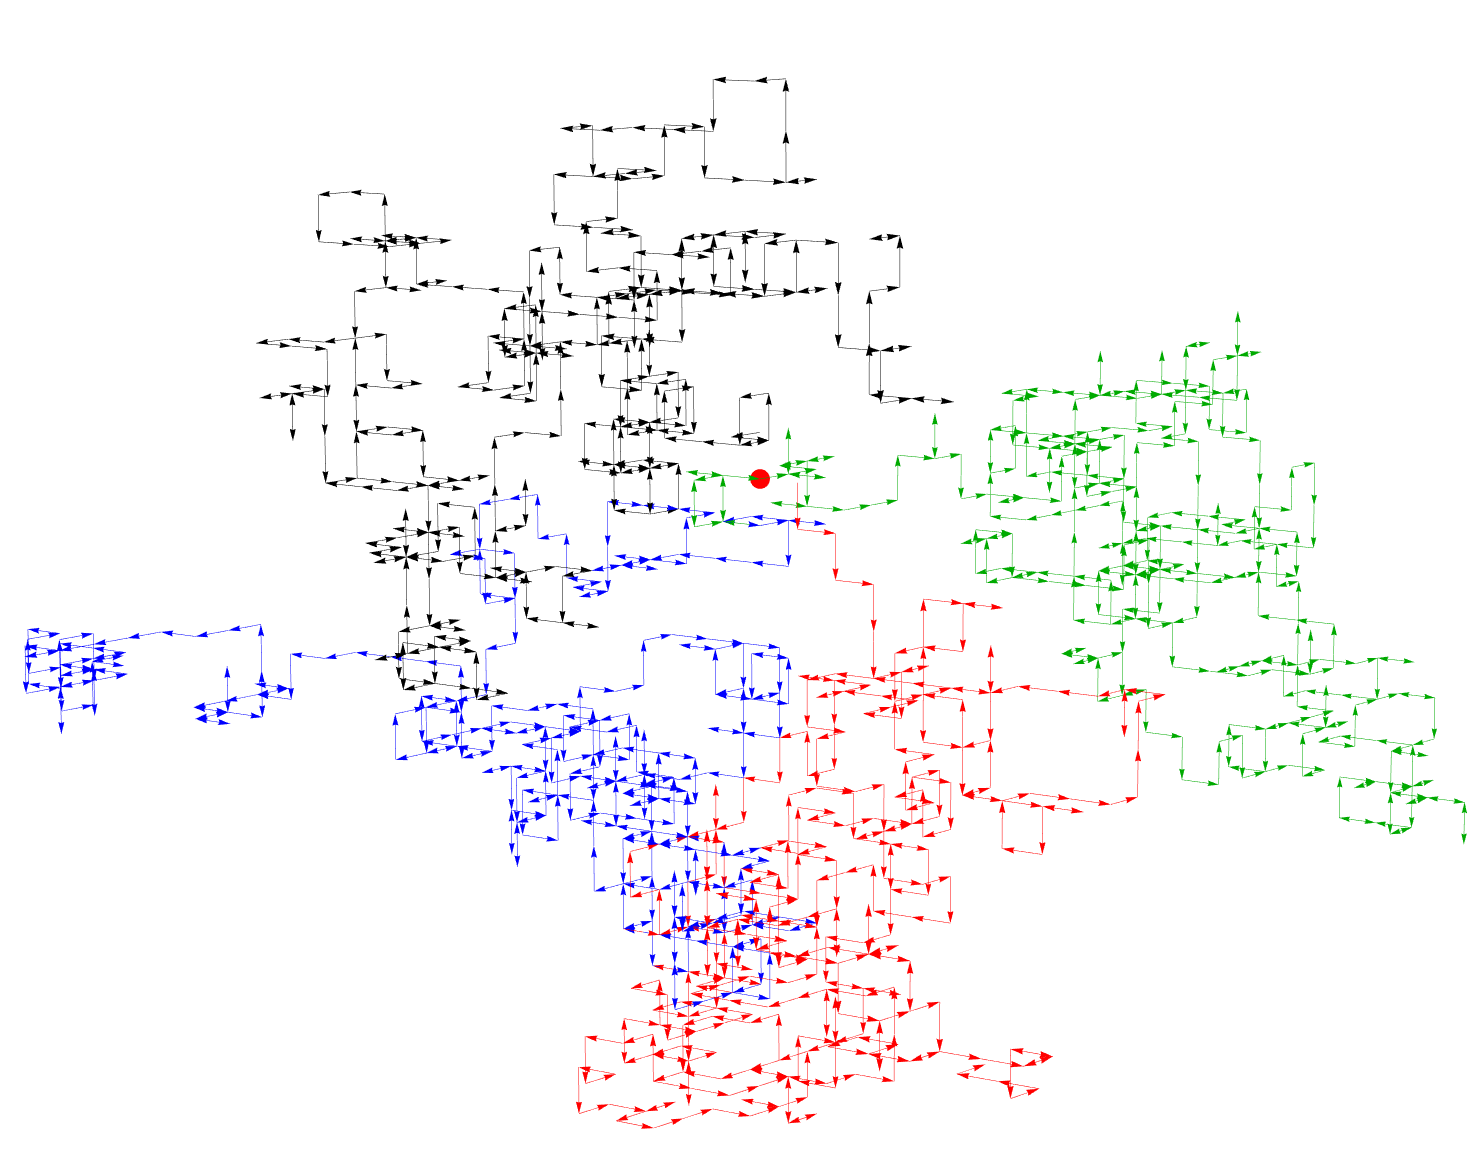
\includegraphics[width=0.8\linewidth]{Figures/quantum-walks/3d-randomwalk.png}
    \caption{Example of three random walks on $\ZZ^3$.}
    \label{fig:intro:3DQWs}
\end{figure}
% \begin{wrapfigure}{r}{10cm}
%     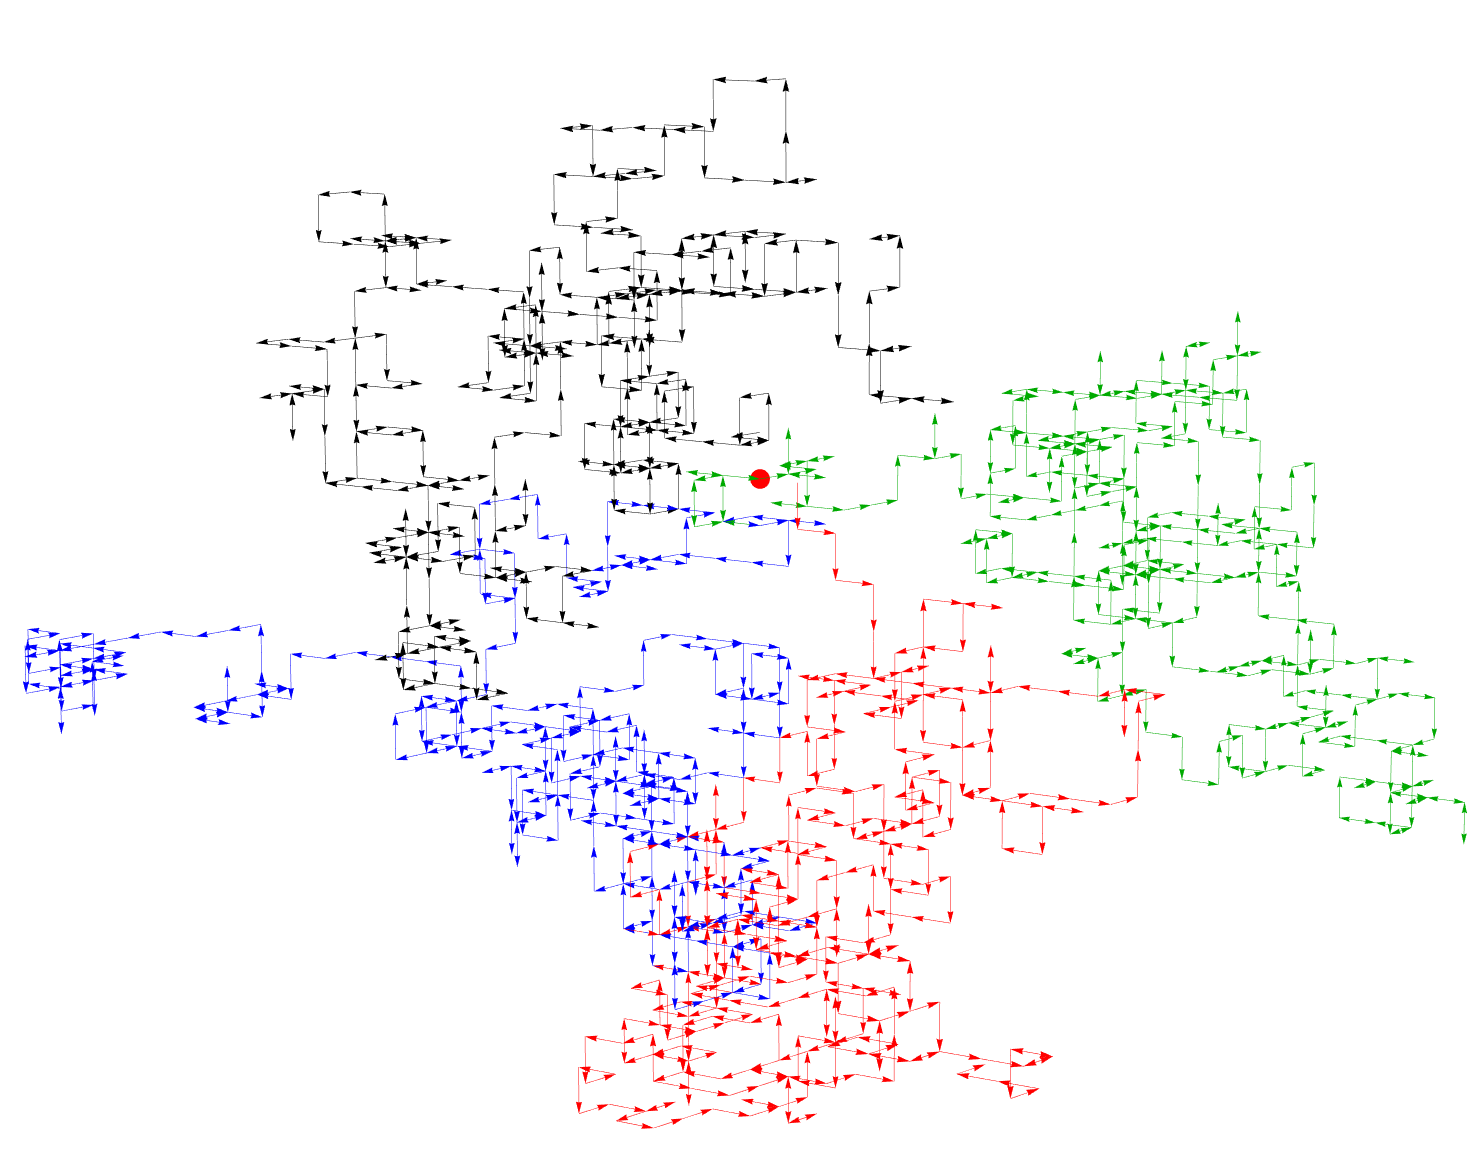
\includegraphics[width=\linewidth]{Figures/quantum-walks/3d-randomwalk.png}
%     \caption{Example of three random walks on $\ZZ^3$.}
% \end{wrapfigure}
% conversionRules = {1 -> {1, 0}, 2 -> {0, 1}, 3 -> {-1, 0}, 
%    4 -> {0, -1}};
% conversionRules3D = {1 -> {1, 0, 0}, 2 -> {0, 1, 0}, 3 -> {0, 0, 1}, 
%    4 -> {0, 0, -1}, 5 -> {0, -1, 0}, 6 -> {-1, 0, 0}};
% makeSteps[num_] := RandomInteger[{1, 4}, num] /. conversionRules;
% makeSteps3D[num_] := RandomInteger[{1, 6}, num] /. conversionRules3D;
% Graphics3D[{
%   {Red, PointSize@0.01, Point@{0, 0, 0}},
%   {Black, Arrowheads@0.005, 
%    Arrow /@ Most@Transpose@{#, RotateLeft@#} &@
%     Accumulate@makeSteps3D@400},
%   {Red, Arrowheads@0.005, 
%    Arrow /@ Most@Transpose@{#, RotateLeft@#} &@
%     Accumulate@makeSteps3D@400},
%   {Blue, Arrowheads@0.005, 
%    Arrow /@ Most@Transpose@{#, RotateLeft@#} &@
%     Accumulate@makeSteps3D@400},
%   {Darker@Green, Arrowheads@0.005, 
%    Arrow /@ Most@Transpose@{#, RotateLeft@#} &@
%     Accumulate@makeSteps3D@400}
%   },
%  (*PlotRange\[Rule]ConstantArray[{-25,25},3],Axes\[Rule]True*)
%  
%  PlotRange -> All, Boxed -> False
%  ]

\tmpHeading{They are time-homogeneous MCs}
The fact that the transition probability does not depend neither on the time $t$ nor on the previous history of the walker, but rather it depends exclusively on the current position, is a crucial properties of random walks, that characterises them as \textit{time-homogeneous Markov chains},
\footnote{A \textit{Markov chain}, or \textit{Markov process}, is a generic type of stochastic process in which the probability of each event only depends on the state of the system at the previous time, rather than on the entire history of the system. Random walks are a notable example of Markov process.}
which is a more general class of memoryless stochastic processes.

\tmpHeading{Transition matrix}
We can collect the set transition probabilities into a matrix $M$. This matrix will then be a \textit{bistochastic matrix}, that is a matrix satisfying $\sum_i M_{ij}=\sum_j M_{ij}=1$. If we collect the set of transition probabilities of going from $i$ to $j$ in the $i$-th column of $M$, we can then write compactly the evolution of a walk in linear algebraic notation as
\begin{equation}
    P_{k+1} = M P_k = M^k P_0,
\end{equation}
where $P_k$ is the vector of probabilities at the set $k$ ($(P_k)_i$ is the probability of finding the walker at the position $i$ at the $k$-th step).

\paragraph{Possible other things to mention here:}
\begin{itemize}
    \item Hitting time
    \item 1D standard example of random walk
    \item Mixing time
    \item Stationary distribution
\end{itemize}


\subsection{Quantum walks}


\tmpHeading{Quantum walks are...}
\acp{QW} are models of quantum dynamics which share similarities with classical random walks, and are therefore often understood as their quantum counterparts.
In its simplest form, a \ac{QW} involves a high-dimensional system (generically a $d$-dimensional system dubbed \textit{qudit}), usually referred to as \emph{walker}, endowed with an inner 2-dimensional degree of freedom, referred to as the \emph{coin state} of the walker. 
At every step, the coin state is \emph{flipped} with some unitary operation, and the walker moves coherently left and right, conditionally on the coin state.
We focus on \acp{DTQW} on a line~\cite{ambainis2001onedimensional}, allowing the coin operation to change from step to step, while remaining site-independent~\cite{ribeiro2004aperiodic,wjcik2004quasiperiodic,bauls2006quantum}.
We demonstrate the effectiveness of this framework for the state engineering of $d$-dimensional systems and provide a set of efficiently verifiable necessary and sufficient conditions for a given state to be the output of a \ac{QW} evolution.	

\tmpHeading{Discrete vs continuous QWs}
A first important distinction is between \textit{discrete} and \textit{continuous} \acp{QW}.
\acp{DTQW} are systems comprised of a low-dimensional degree of freedom, usually referred to as the \textit{coin}, coupled with a high-dimensional one named the \textit{walker}.
In this model, the time is discrete in the sense that the state evolves in discrete \textit{jumps}, rather than evolving continuously in time.
A different model is the so-called \ac{CTQW}. Here, the dynamics is instead governed by a standard Schr\"odinger equation, and the process is therefore defined via some Hamiltonian. In a \ac{CTQW} there is no place for the notion of a \textit{coin} degree of freedom, which makes the structure of these kinds of model rather different, at least on the surface, from their discrete counterparts\highlight{(maybe mention equivalence between discrete and continuous models)}.

\tmpHeading{(QWs for quantum algorithms?)}
\acp{QW} have also been proven to be useful to develop quantum algorithms, and it was recently proved that \acp{QW} are universal for quantum compuation~\cite{childs2009universal,childs2003exponential,lovett2010universal,lovett2018quantum,underwood2010universal}.
Reviews of QW-based quantum search algorithms~\cite{ambainis2011search,ambainis2008quantum,ambainis2010developments,kempe2003quantum,kendon2006random,santha2008quantum,venegasandraca2012quantum,venegasandraca2008quantum}.

\subsection{DTQWs}

\acp{DTQW} share many features with classical random walks.
In particular, like the classical case, they come with a notion of a \textit{coin}: a random choice that is made at every step and determines the direction in which the walker moves.
In the \ac{QW}, the coin becomes a quantum state, often but not necessarily a two-dimensional one, and the coin flipping operation becomes a unitary operation applied to the coin state.
The walker also becomes a quantum state, typically of dimension much higher than the coin state. At every step, the walker's state changes conditionally to the state of the coin after the coin flipping operation.
In contrast with the classical case, the evolution is here \textit{coherent}, bringing interference effects into the picture, which allows for features not found in the standard random walk model.

A single \textit{step} of a \ac{DTQW} consists of a unitary evolution applied to the current state of the \ac{QW}.
The time is therefore here \textit{discrete} in the sense that there is no real notion of ``time'' as a continuous parameter. Rather, the state changes by discrete amounts at every step, just as its classical counterpart.

We will focus here on the simplest type of \ac{DTQW} model, in which the coin is a two-dimensional state and the walker is some high-dimensional state.
In this model, the evolving state lives in a Hilbert space $\calH\equiv\calH_C\otimes\calH_W$, with $\calH_C$ the two-dimensional space of the coin, and $\calH_W$ an high-dimensional space accomodating the possible states of the walker.
A generic state for a DTQW can be written as
\begin{equation}
    \ket\Psi = \sum_j \sum_{s\in\{0,1\}} c_{j,s} \ket{s, j},
\end{equation}
for some coefficients $c_{j,s}\in\CC$, and with the index $j$ spanning the possible values of the walker.
The evolution of the \ac{DTQW} is a two-step process.
First, a unitary operation is applied locally to the coin.
Then, a controlled-shift operation is applied to the walker, changing its state conditionally to that of the coin.
Formally, we write a single \textit{step operator} as $\calW=\calS\calC$, with $\calS,\calC\in\Lin(\calH)$ and $\calC\equiv\calC\otimes I_W$\footnote{More precisely, this means that $\calC=\calC\otimes I_W$}.
The shift operator $\calS$ is usually written in the form
\begin{equation}
    \calS = \PP_0\otimes \EE_+ + \PP_1\otimes \EE_-,
    \label{eq:qws_shitty_definition_cshift}
\end{equation}
where $\PP_k\equiv\ketbra k$ and $\EE_\pm$ are operators moving the walker in one direction or the other:
\begin{equation}
    \EE_+\equiv \sum_k \ketbra{k+1}{k},
    \qquad
    \EE_-\equiv\sum_k\ketbra{k}{k+1}.
\end{equation}
The choice of coin operation $\calC$ is what defines a particular DTQW.
A standard choice is to use a \textit{Hadamard coin}, that is, $\calC=H$ where $H$ is the Hadamard matrix, defined via its action on the computational basis as
$H\ket0=\ket+$ and $H\ket1=\ket-$, where $\ket\pm\equiv\frac{1}{\sqrt2}(\ket0\pm\ket1)$.

\begin{example}[label=ex:hadamard_walk]
As an example, consider what happens with an initial state $\ket{\Psi_0}\equiv\ket{\uparrow,0}$, writing for ease of notation write the coin states as $\uparrow,\downarrow$ instead of $0$ and $1$.
The first coin operation sends this to $\ket{+,0}\equiv\frac{1}{\sqrt2}(\ket0+\ket1)$, after which the shift $\calS$ gives
\begin{equation}
    \ket{\Psi_1} \equiv 
    \calS\calC\ket{\Psi_0} =
    \calS\ket{+,0} =
    \frac{1}{\sqrt2} \left( \ket{\uparrow,+1} + \ket{\downarrow, -1} \right).
\end{equation}
The next step then sends this into
\begin{equation}
    \ket{\Psi_2} \equiv
    \frac12\left[
        \ket{\uparrow,+2} +
        (\ket{\downarrow}
        + \ket{\uparrow})\otimes \ket{0}
        - \ket{\downarrow, -2}
    \right],
\end{equation}
and then at the third step,
\begin{equation}
    \ket{\Psi_3} \equiv
    \frac{1}{2\sqrt2}\left[
        \ket{\uparrow,+3} +
        (\ket{\downarrow} + 2\ket{\uparrow})\otimes \ket{+1}
        - \ket{\uparrow,-1}
        + \ket{\downarrow,-3}
    \right].
\end{equation}
The calculation proceeds similarly for larger numbers of steps.
Note how the walker proceeds asymmetrically, even though the direct classical analogue of an Hadamard walk would be a random walk with equal probabilities of going left or right at every step.
The reason for this is in the interference effects, and the fact that the Hadamard treats $\ket\uparrow$ and $\ket\downarrow$ asymmetrically.
See~\cref{fig:hadamardwalk_Nsteps} for a simulation of the Hadamard walk with $20$ and $40$ steps, which shows clearly the asymmetry present in the output states.
\end{example}

\tmpHeading{A more efficient formalism for DTQWs}
One feature that emerges clearly from the above example is that, at each step, some of the possible walker's position are never occupied. More precisely, if we start with the walker at a single fixed position, say the position $\ket0$, then at odd-numbered steps only even positions will have nonzero probability amplitudes.
This symmetry can be exploited to make simulations more efficient, as well as simplify the derived expression removing modes that we know are never going to be occupied.
We will then in the following use a variation of~\cref{eq:qws_shitty_definition_cshift} in which instead of having the walker move either left or right, we have the walker either stay still or moving in one direction (say, right):
\begin{equation}
    \calS = \PP_0\otimes I + \PP_1\otimes \EE_+
    =\ketbra0\otimes I +\ketbra1\otimes\sum_k\ketbra{k+1}{k}.
\end{equation}
This notation, while somewhat nonstandard, has proven useful in some works~\cite{hoyer2009faster,montero2013unidirectional,montero2015quantum}, and will be used in~\cref{sec:intro:QWs} to obtain most of our analytical results.

\begin{figure}[tb]
    \centering
    \subfloat[$20$ steps]{{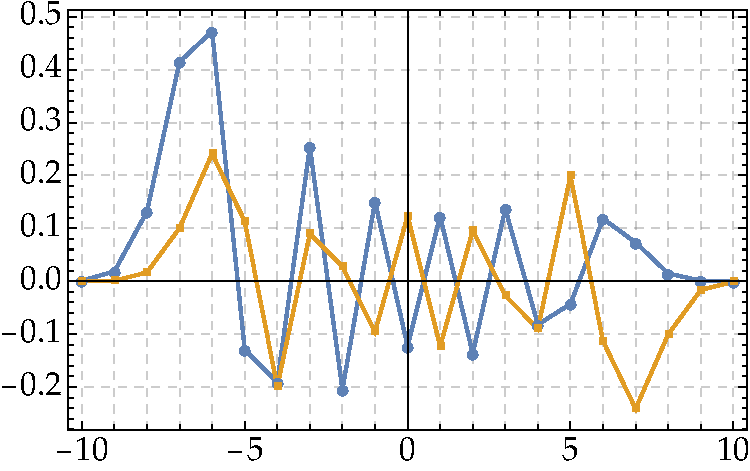
\includegraphics[width=.4\linewidth]{QW20steps_initstateUp} }}%
    \qquad
    \subfloat[$40$ steps]{{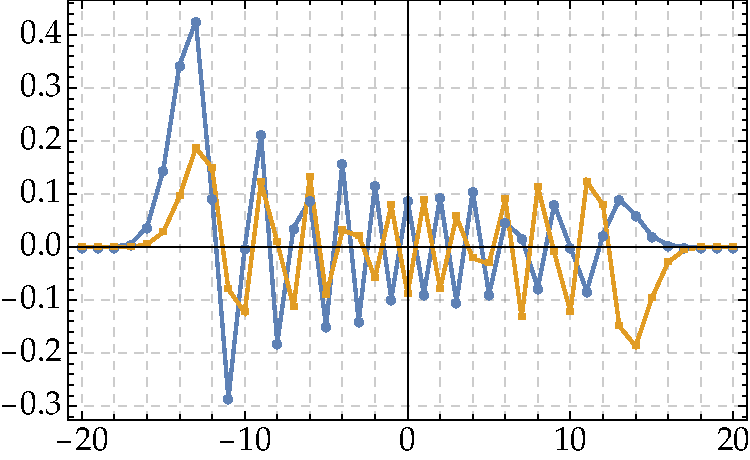
\includegraphics[width=.4\linewidth]{QW40steps_initstateUp} }}%
    % 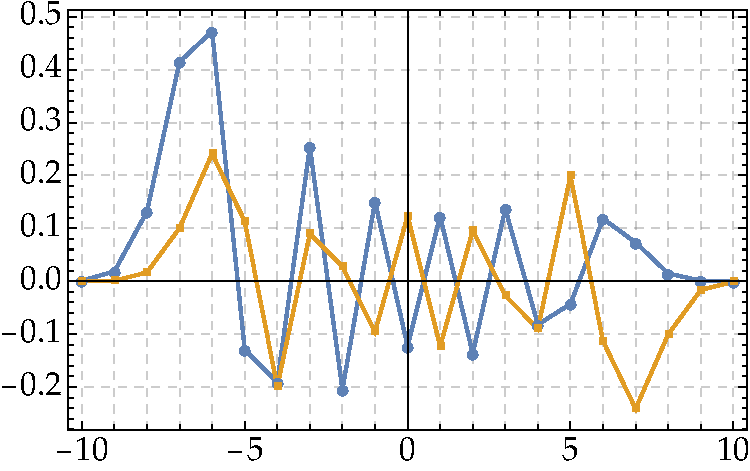
\includegraphics[width=.5\linewidth]{QW20steps_initstateUp}
    \caption{
        Output amplitudes of $20$ steps of Hadamard walk, with initial state $\ket{\Psi_0}\equiv\ket{\uparrow,0}$.
        Blue (circles) and orange (squares) points are the output amplitudes corresponding to the coin state $\ket\uparrow$ and $\ket\downarrow$, respectively.
    }
    \label{fig:hadamardwalk_Nsteps}
\end{figure}
% reindexForQW[amps_] := Transpose[
%    {{#[[1]], #[[2, 1]]}, {#[[1]], #[[2, 2]]}} & /@ 
%       Thread@{Range@Length@# - 1/2 - Length@#/2, #} &@amps
%    ];
% outAmps = 
%   QWEvolve[{1., 0}, ConstantArray[{\[Pi]/4, \[Pi]/2, \[Pi]/2}, 20], 
%     "SimulationMethod" -> "StepByStep"] // Partition[#, 2] &;
% fig = ListPlot[reindexForQW@outAmps, Joined -> True, 
%   PlotMarkers -> Automatic, Frame -> True, 
%   GridLines -> {Range[-20, 20], Range[-1, 1, 0.1]},
%   GridLinesStyle -> Directive[Opacity@.4, Gray, Dashed],
%   FrameStyle -> 
%    Directive[Black, FontFamily -> "TeX Gyre Pagella Math", 
%     FontSize -> 16]
%   ]



